\documentclass[]{aastex63}

\usepackage{graphicx}
%\graphicspath{{.}} %Setting the graphicspath
\usepackage{advdate}
\usepackage{amsmath}
\usepackage{appendix}

\newcommand{\asec}{\hbox to 1pt{}\rlap{$^{\prime\prime}$}.\hbox to 2pt{}}
\newcommand{\amin}{\hbox to 1pt{}\rlap{$^{\prime}$}.\hbox to 1pt{}}
\newcommand{\adeg}{\hbox to 1pt{}\rlap{$^{\circ}$}.\hbox to 2pt{}}
\newcommand{\trl}{\color{red} }
\newcommand{\dhm}{\color{blue} }

% Macros for DHM vector notation
\newcommand{\BV}[1]{\mathbf{#1}}
\newcommand{\BH}[1]{\hat{\mathbf{#1}}}
\newcommand{\BL}{\boldsymbol{\Lambda}}
\newcommand{\cross}{\boldsymbol{\times}}
% End DHM macros

\begin{document}

\subsection{The Navigation Methodology}

Fig.(\ref{fig:nav_wide}) diagrams the basic geometry of interstellar navigation.  We know with great precision the position vectors $\BV{p_k}$ of nearby stars in three dimensions from the Gaia DR3 archive.  (We'll return to exactly how precise later.)  We measure the apparent directions to those stars - unit vectors $\BH{d}_k$ - from the vantage point of a spacecraft.  Each such measurement constrains the spacecraft to lie on the sight line in the direction $\BH{d}_k$ passing through the point $\BV{p}_k,$ therefore measuring the directions to two or more stars constrains the spacecraft to lie at the point where all these lines intersect.

In practice, the lines will all be skew (that is, non-intersecting), and we are faced with the more nebulous job of describing the position and shape of the region of space where the spacecraft must be located in order to be consistent with all our direction measurements. Fig.(\ref{fig:nav_wide}) hints at this problem with dotted lines on either side of the star sight lines showing the transverse displacements of the lines if our direction measurements had differed by $1''$ of arc.  In fact, the transverse displacement of each line in au is numerically equal to the distance to the corresponding star in pc!  We usually think of 1~pc as the distance of a star for which a 1~au displacement of the observer changes its direction by $1''$, but for navigation problems, we think of it as the distance for which a $1''$ change in direction causes a 1~au transverse displacement of the sight line.  A parsec is an au per arcsecond.  Of course, our actual angular errors are not $1''$ - in fact, Fig.(\ref{fig:nav_wide}) shows we do much better - so the spacecraft must actually be in a region with dimensions scaled by the ratio of our actual angle errors to $1''.$

\begin{figure}[hbtp]
\centering
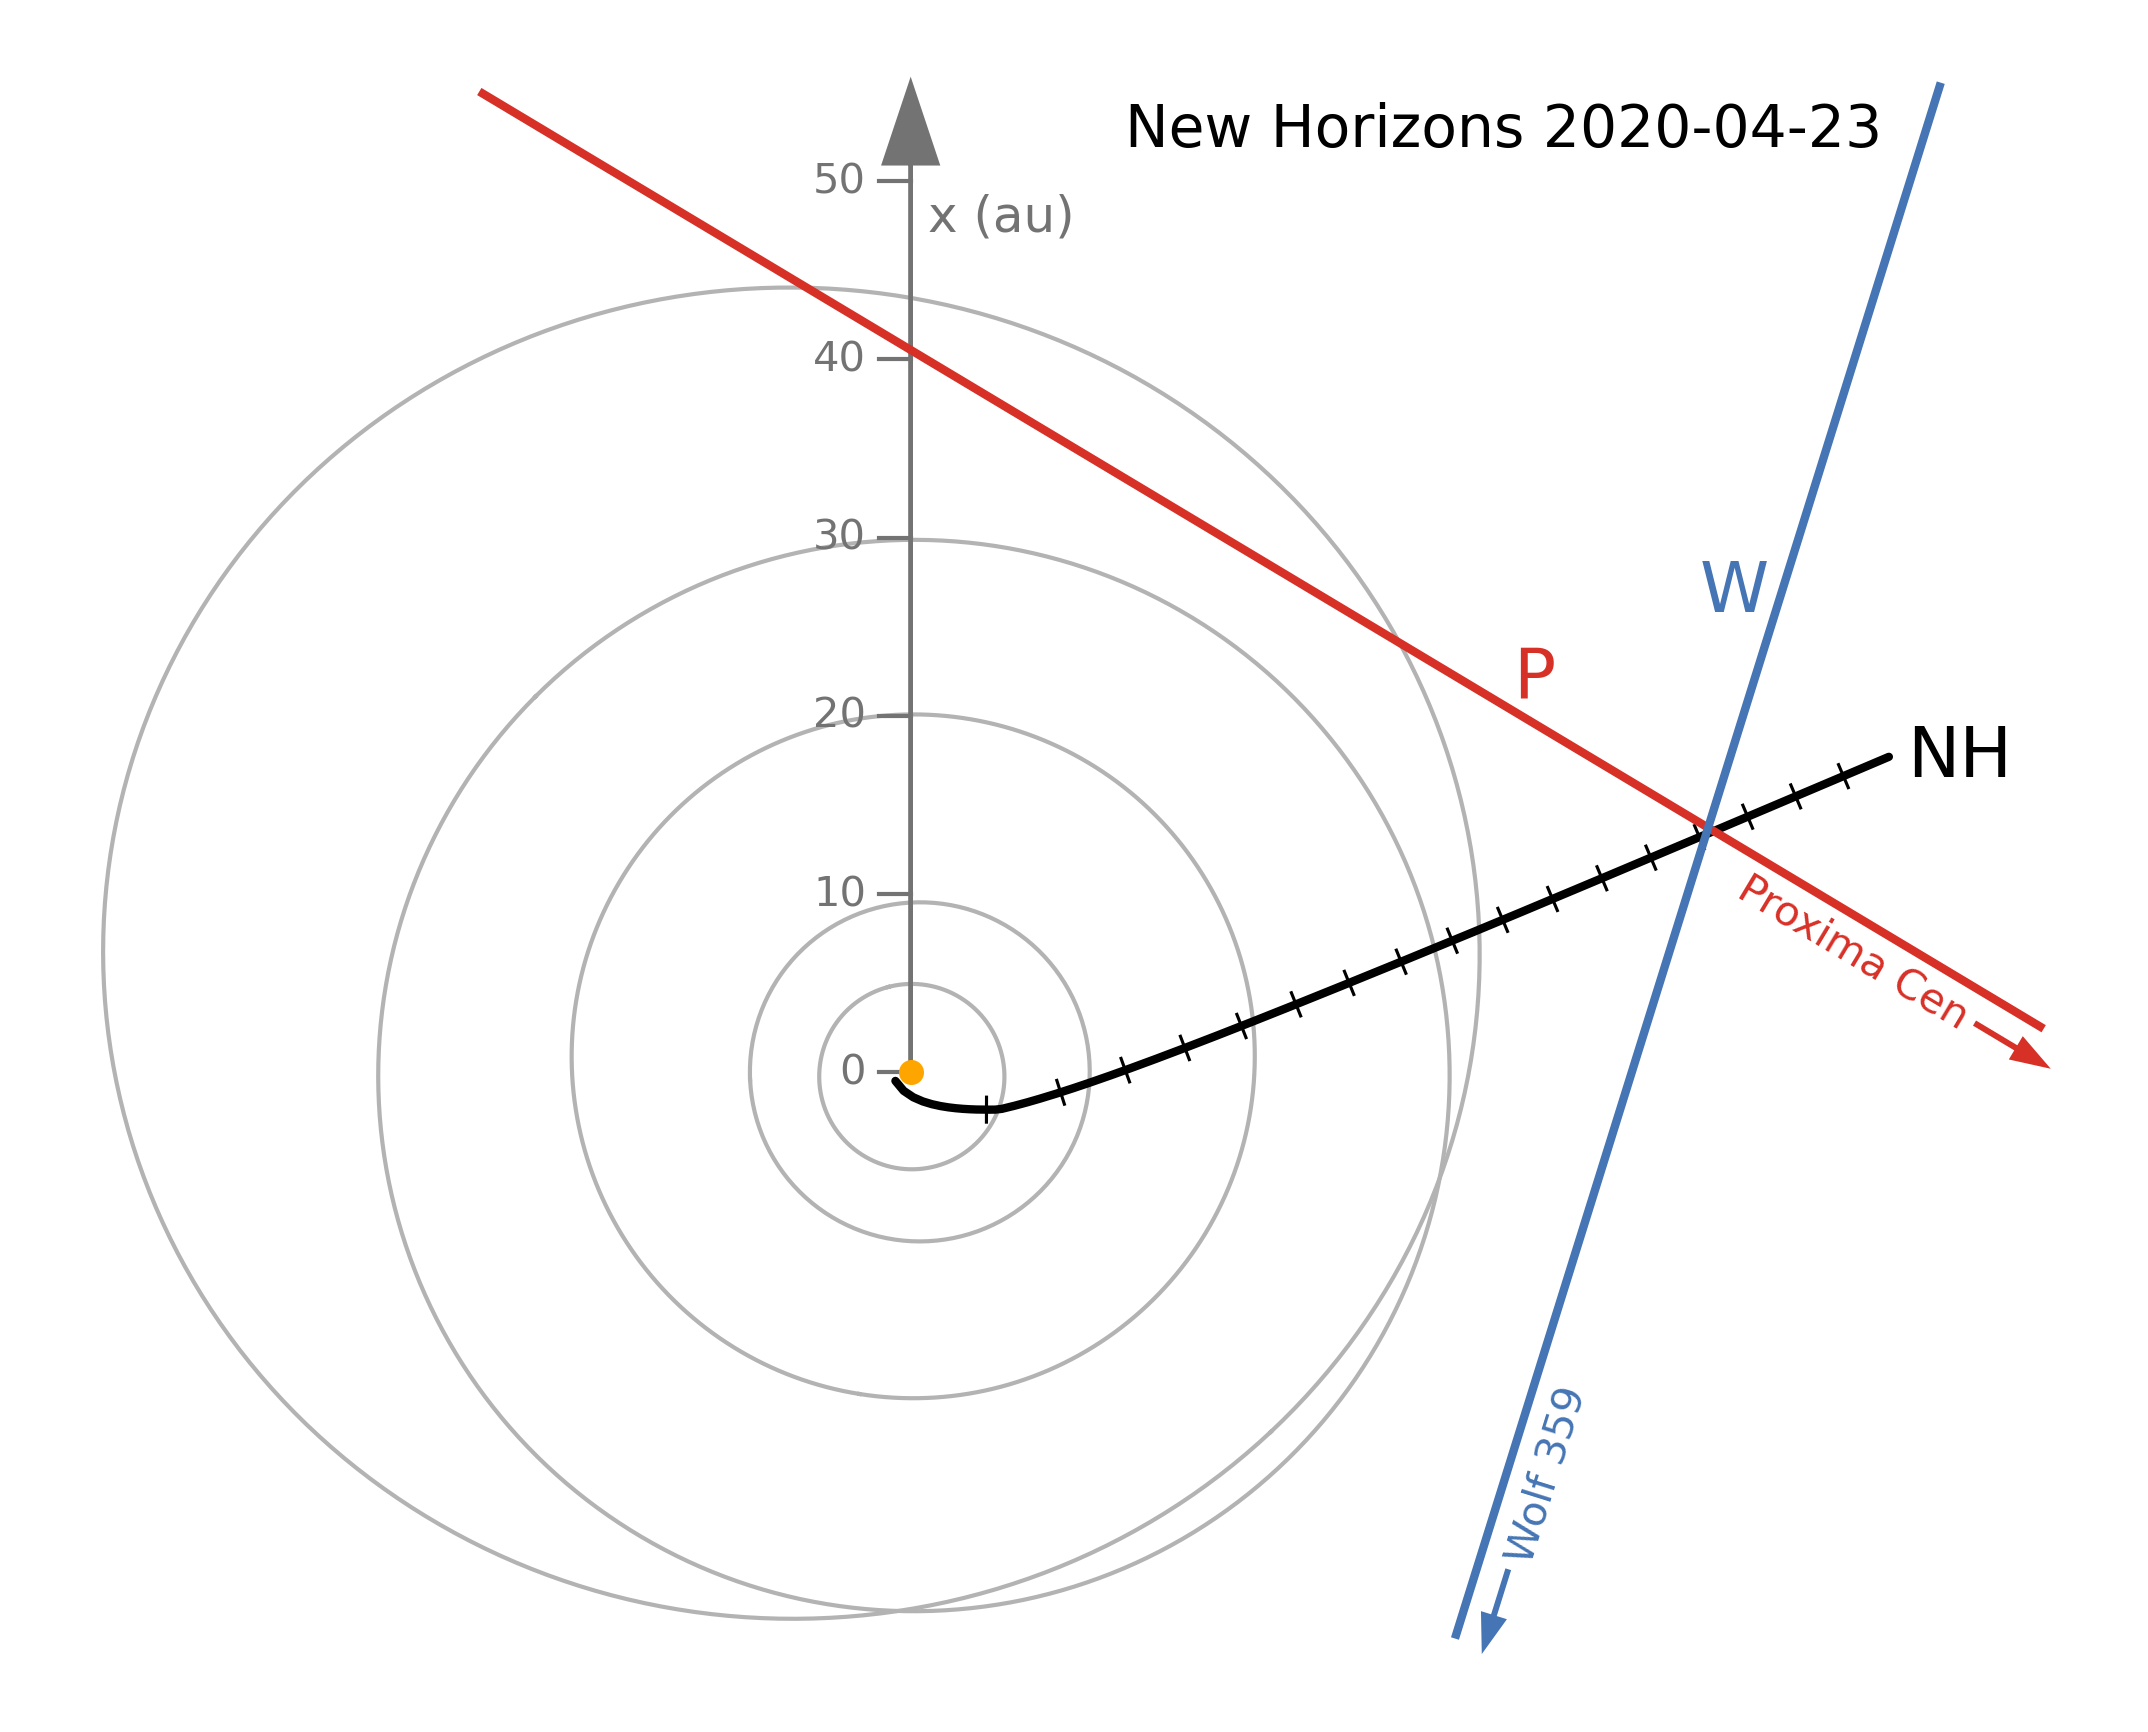
\includegraphics[keepaspectratio,width=5.0 in]{nhfig1.png}
\caption{The location of New Horizons on 2020 April 23 as derived from the directions to Proxima Cen and Wolf 359 measured from the spacecraft.  This is the view from the ecliptic north pole; the vertical axis is at zero right ascension and the origin is the solar system barycenter.  The line P passes through the precise GAIA 3-D location of Proxima Cen, in the direction measured from the spacecraft.  In other words, the LORRI image of Proxima Cen constrains the spacecraft to lie on line P. Similarly, the LORRI image of Wolf 359 constrains the spacecraft to lie on line W.  The adjacent faint dotted lines show how much P and W would be displaced by a $1''$ change in line direction; the transverse displacement in au is just the distance to the star in pc (1.30 for P, 2.41 for W). The trajectory NH is the actual path of the spacecraft from launch in 2006 through 2023, with ticks on January 1 each year.  Notice that our actual angular errors must be much less than the $1''$ indicated by the dotted lines.  Proxima Cen is $\sim 45^\circ$ south of the ecliptic, so line P tilts into the page at that angle; Wolf 359 and the NH trajectory are within $2^\circ$ of the ecliptic.}
\label{fig:nav_wide}
\end{figure}

The dotted lines in Fig.(\ref{fig:nav_wide}) really represent the standard deviation of cylindrical Gaussian probability clouds around the lines P and W.  Our measurements constrain the spacecraft to the ellipsoidal Gaussian probability cloud that is the product of the individual cylindrical distributions.  You can see the projected shape of this error ellipsoid in the parallelogram where the dotted lines in Fig.(\ref{fig:nav_wide}) cross (scaled up in size as if our angular errors were $1''$) - just picture the ellipse inscribed in that parallelogram.  Given our measurements, the center of this error ellipsoid is the most likely position of our spacecraft, in other words our best guess at $\BV{x}$ given the directions we measured. The shape and size of the error ellipsoid are our estimate of the uncertainty in our derived position $\BV{x}.$

If the actual spacecraft position is $\BV{x},$ then the actual direction to star $k$ is $(\BV{x}-\BV{p}_k)/|\BV{x}-\BV{p}_k|.$ (These are the GAA+JPL entries in Table 2.)  Let $\delta\alpha_k$ be the angle between this and our measured direction $\BH{d}_k$ - our measurement error.  Writing $p_k$ for $|\BV{p}_k|,$ then since $\delta\alpha_k$ and $|\BV{x}|/p_k$ are both very small,
\begin{equation*} \delta\alpha_k =
  |\BH{d}_k\cross(\BV{x}-\BV{p}_k)|/p_k,
\end{equation*}
which we rewrite as
\begin{equation} \delta\alpha_k^2 = \bigl(|\BV{x}-\BV{p}_k|^2 -
  (\BH{d}_k\cdot(\BV{x}-\BV{p}_k))^2\bigr)/p_k^2.
\label{eq:alpha2}\end{equation}
If our measurements all have the same standard errors in angle, say $\sigma_\alpha,$ then each cylindrical Gaussian cloud will be $\exp(-\tfrac{1}{2}\delta\alpha_k^2/\sigma_\alpha^2),$ so the combined ellipsoidal cloud will be $\exp(-\tfrac{1}{2}\chi^2),$ where
\begin{equation} \chi^2 = \sum_k\delta\alpha_k^2/\sigma_\alpha^2.
\label{eq:chi2}\end{equation}
The center of this cloud is where $\chi^2$ is minimum, which is a perfectly well-defined point $\BV{x}$ even when the lines do not exactly meet (that is, when $\chi^2$ never reaches zero).

What we are describing here is the well-known minimum chi-squared technique for finding the most likely parameters consistent with a set of measurements.  Here, $\chi^2$ is quadratic in $\BV{x},$ so setting its gradient to zero to find its minimum produces a simple $3\times 3$ system of linear equations for $\BV{x}.$ The gradient of Eq.(\ref{eq:alpha2}) is
\begin{align*}
  \nabla\delta\alpha_k^2&= (2/p_k^2)\bigl((\BV{x}-\BV{p}_k)
                          - \BH{d}_k\BH{d}_k\cdot(\BV{x}-\BV{p}_k)\bigr) \\
                        &= (2/p_k^2)\BV{Q}_k(\BV{x}-\BV{p}_k),
\end{align*}
where we have defined $\BV{Q}_k=\BV{I}-\BH{d}_k\BH{d}_k^T$ as the $3\times 3$ matrix which projects vectors into the plane perpendicular to $\BH{d}_k.$  Setting $\nabla\chi^2=0$ and solving for $\BV{x}$ gives
\begin{equation} \BV{x} = \BL^{-1}\sum_k\BV{Q}_k\BV{p}_k/p_k^2,
\label{eq:x}\end{equation}
where
\begin{equation} \BL = \sum_k\BV{Q}_k/p_k^2.
\label{eq:xlambda}\end{equation}

Eq.(\ref{eq:alpha2}) looks simpler when expressed in matrix notation using the $\BV{Q}_k$ projection operator, so we can rewrite Eq.(\ref{eq:chi2}) as
\begin{equation} \chi^2 = (1/\sigma_\alpha^2)
  \sum_k(\BV{x}-\BV{p}_k)^T\BV{Q}_k(\BV{x}-\BV{p}_k)/p_k^2.
\label{eq:chi2a}\end{equation}
Now $\chi^2$ is just a quadratic in $\BV{x},$ and its second degree terms are proportional to $\BV{x}^T\bigl(\sum_k\BV{Q}_k/p_k^2\bigr)\BV{x},$ or $\BV{x}^T\BL \BV{x}.$ By construction, $\BL$ is a symmetric positive definite $3\times 3$ matrix, so its eigenvalues are positive and its eigenvectors form an orthogonal basis.  Since the ellipsoidal probability distribution for $\BV{x}$ is $\exp(-\tfrac{1}{2}\chi^2),$ those eigenvectors are the principal axes of the error ellipsoid, and the corresponding eigenvalues are the squares of its semi-axes.  Thus,
\begin{equation} \BV{V}_\BV{x} = \sigma_\alpha^2\BL^{-1} =
  \sigma_\alpha^2\bigl(\sum_k\BV{Q}_k/p_k^2\bigr)^{-1}
\label{eq:xcov}\end{equation}
is the covariance matrix for for our most likely spacecraft position $\BV{x}$ given by Eq.(\ref{eq:x}).  Its eigenvalues (or singular values) are the squares of the principal axes of the error ellipsoid for the spacecraft position $\BV{x}$ calculated using Eq.(\ref{eq:x}).  Note that if $p_k$ are in parsecs and $\sigma_\alpha$ is in arcseconds, then the units of $\BV{V}_\BV{x}$ will be au$^2.$ Eq.(\ref{eq:xcov}) is a sort of matrix harmonic mean of the $p_k^2,$ with the $\BV{Q}_k$ projection matrices providing weighting to account for the angles among the stars.

Eq.(\ref{eq:x}) matches the formulas given in Kaplan [2011], with the $1/p_k^2$ providing the weights for the terms in the sum.  [More here.]

To estimate the error $\sigma_\alpha$ in extracting the direction of a star from a particular LORRI image is not easy, and the error will certainly vary from image to image depending on the exact circumstances of spacecraft residual slew rates, exposure times, the background star field, and many other factors.  Many of these factors will not be known until after the image has been made, so for the purposes of planning a set of observations, a reasonable assumption is that the error in $\BH{d}_k$ is simply some angle $\sigma_\alpha$ on the sky.  For a star at distance $p_k$ (in pc) an error $\sigma_\alpha$ (in $''$) will cause the line determined by $\BH{d}_k$ and $\BV{p}_k$ to be displaced by $p_k\sigma_\alpha$.  For a single LORRI image, experience has shown us that $\sigma_\alpha$ is of order $0''\!\!.2$ (1~$\mu$rad).  A single pixel is $4''\!\!.08$, so this amounts to 0.05 pixel.  Note that this is not a question of the resolution of the instrument, but of how well one statistic - the centroid - can be determined for something known to be a point source. This is very much a ballpark estimate, within perhaps a factor of two or three.

We have been ignoring any errors in the Gaia DR3 data for good reason. Typical Gaia position errors are of order $0''\!\!.00003$ at its baseline J2016.0 epoch, although errors in Gaia proper motions very rapidly degrade this accuracy over the 4.3~yr interval to April 2020, at least for high proper motion stars like Proxima Cen and Wolf 359. For them, the Gaia position errors have dropped to of order $0''\!\!.0003$ - but that is still a factor of a thousand less than $\sigma_\alpha.$ Gaia parallax errors are also of order $0''\!\!.00005,$ causing an uncertainty in $p_k$ of about 20~au for Proxima Cen, and 80~au for Wolf 359.  These differences are projected transverse to the line of sight from the spacecraft by the same tiny angle of a few seconds of arc shown in Fig.(1) and Fig.(2), again causing a completely negligible uncertainty in the transverse displacement of line P or W in Fig.(\ref{fig:nav_wide}).

Although the angular error in the direction measurement for a single LORRI image is of order $0''\!\!.2,$ we routinely reduce this error by averaging the measurements from several images of the same target.  In this case, we made six images each of Proxima Cen and Wolf 359, which we believe reduces $\sigma_\alpha$ by a factor of $\sqrt{6},$ to a bit under $0''\!\!.1$ or 0.025 pixel.  Eventually, systematic errors and drifts will put a halt to this improvement, but for the case of LORRI, we are not sure what the best acheivable $\sigma_\alpha$ might be.

We have aggregated our six images of each star into a single direction measurement for the purposes of the plot in Fig.(\ref{fig:nav_zoom}), but we point out that Eq.(\ref{eq:x}) and Eq.(\ref{eq:xcov}) produce exactly the same values of both $\BV{x}$ and its covariance matrix (error ellipsoid) $\BV{V}_\BV{x}$ if you feed the directions of all twelve images into them, as if they were $N=12$ individual stars.  That is, $\BV{x}$ for this $N=12$ set of directions will be exactly the same as if you had used the mean $\BH{d}_k$ from the six images of the same star in an $N=2$ application of Eq.(\ref{eq:x}).  Similarly, an $N=12$ version of Eq.(\ref{eq:xcov}) will produce the same error ellipsoid as the $N=2$ version with $\sigma_\alpha$ reduced by $\sqrt{6}.$

The size and shape of the error ellipse given by Eq.(\ref{eq:xcov}) can also be used as a design tool to develop an observational program for locating a spacecraft.  Since the accuracy of the derived position is directly proportional to the distance of the star, only a few of the nearest stars are realistic candidates for this purpose.  Using Eq.(\ref{eq:xcov}), you can rank all of the pairs of these navigation candidate stars by their performance in constraining spacecraft position.  To do this, you set $\BH{d}_k$ equal to $\BV{p}_k/p_k$ (a very good approximation), and do a singular value decomposition of the resulting $\BV{V}_\BV{x}/\sigma_\alpha^2$ matrix. The square roots of the largest and smallest singular values are the shortest and longest axes of the error ellipse for a position determination based on the directions of that pair of stars.  The best pair for determining spacecraft positon will be the one with the smallest long axis.  If you put in the $p_k$ in units of pc, the error ellipse axis will be in au per arcsecond of $\sigma_\alpha.$ Table 4x shows all five of the navigational candidate stars within 3~pc and the performance of all ten pairs of them.

\begin{deluxetable}{lrrrrcccccr}
\tabletypesize{\small}
\tablecolumns{11}
\tablewidth{0pt}
\tablecaption{Candidate Navigation Stars}
\tablehead{
  \colhead{}&\colhead{}&\colhead{}&\colhead{}&\colhead{}
  & \multicolumn{5}{c}{Pair Ellipsoid Axes (au/as)} & \colhead{} \\
\multicolumn{1}{l}{Star} &
\multicolumn{1}{c}{RA} &
\multicolumn{1}{c}{DEC} &
\multicolumn{1}{c}{V(mag)} &
\multicolumn{1}{c}{r(pc)} &
\multicolumn{1}{c}{P} &
\multicolumn{1}{c}{B} &
\multicolumn{1}{c}{W} &
\multicolumn{1}{c}{H} &
\multicolumn{1}{c}{C} &
\multicolumn{1}{c}{NH}
}
\startdata
Proxima Cen (P)   &217$^\circ$&-63$^\circ$& 11.1& 1.30&     & 1.06& 1.15& 1.16& 1.19&  63$^\circ$ \\
Barnard's Star (B)&269$^\circ$&  5$^\circ$&  9.5& 1.83& 1.91&     & 1.46& 1.49& 1.56&  31$^\circ$ \\
Wolf 359 (W)      &164$^\circ$&  7$^\circ$& 13.5& 2.41& 2.45& 2.58&     & 1.75& 1.87& 124$^\circ$ \\
HD 95735 (H)      &166$^\circ$& 36$^\circ$&  7.5& 2.55& 2.70& 2.60& 7.00&     & 1.93& 127$^\circ$ \\
CD-23 14742 (C)   &282$^\circ$&-24$^\circ$& 10.4& 2.98& 3.64& 6.54& 3.80& 4.24&     &   6° \\
\enddata
\tablecomments{Candidate navigation stars within 3 pc.  (The other three stars within 3 pc are Alpha Cen, Sirius, and UV Ceti, excluded here because they are multiple star systems.  Sirius and Alpha Cen are also too bright.)  The Pair Ellipsoid Axes columns are the largest (below diagonal) and smallest (above diagonal) axes of the error ellipsoid computed using Eq.(\ref{eq:xcov}) for the corresponding pair.  The NH column shows the angle of the star from the SSB-New Horizons direction, which was a separate criterion for the parallax program of the present study discussed in section 2.}
\end{deluxetable}\label{tab:navstars}

We originally thought that increasing the number of different stars would be important to improve the accuracy of a position determination based on observations of their directions.  However, Eq.(\ref{eq:xcov}) tells a different story.  You can also use it to rank the relative performance of three or four or any number of stars according to the size of the error ellipse they produce.  When we did this, we discovered that it is almost always better to repeat an image of a closer star that you have already used, than to add an image of a new more distant star.  This is certainly true of Proxima Cen and Wolf 359: If you want to improve the accuracy of $\BV{x}$ by choosing a third star to image, your very best option among all the stars in the sky is to repeat your direction measurement of Wolf 359.  The resulting reduction in the longest axis of your error ellipse will be better than any other star.  For navigation purposes, your optimal strategy is to choose the best pair of stars you can, and image them over and over to beat down their effective $\sigma_\alpha.$

\subsection{The Derived Position of New Horizons}

Fig.(\ref{fig:nav_zoom}) shows in detail what happened when we applied this methodology to our Proxima Cen and Wolf 359 direction measurements.  On the left is a zoomed-in view of the same geomtery depicted in Fig.(\ref{fig:nav_wide}), viewed in the measured direction of Proxima Cen, so that the line P has been reduced to a point.  On the right is the analogous view at the same scale in the direction of Wolf 359, reducing the line W to a point.  These are the aggregated lines, so the directions $\BH{d}_k$ are the means of the directions measured in the six individual images of each star.  The faint dotted circles and lines are at multiples of $0''\!\!.1$ from the P and W lines; recall that our estimated $\sigma_\alpha$ is a bit less than this at $0''\!\!.2/\sqrt{6}=0''\!\!.087.$ The star marks our best estimate of the spacecraft position $\BV{x}$ from Eq.(\ref{eq:x}).  The actual spacecraft position on April 23, 2020 according to JPL is at the intersection of the two gray axes.  It is 0.350~au away from the starred position derived from our LORRI images. The solid ellipses are the 1-sigma and 2-sigma error ellipses from Eq.(\ref{eq:xcov}).  The actual position is near the 2-sigma error ellipse, which probably means that our assumed $0''\!\!.2$ error for a single LORRI image is too optimistic - it may be nearer 0.1 pixel than 0.05 pixel.

\begin{figure}[hbtp]
\centering
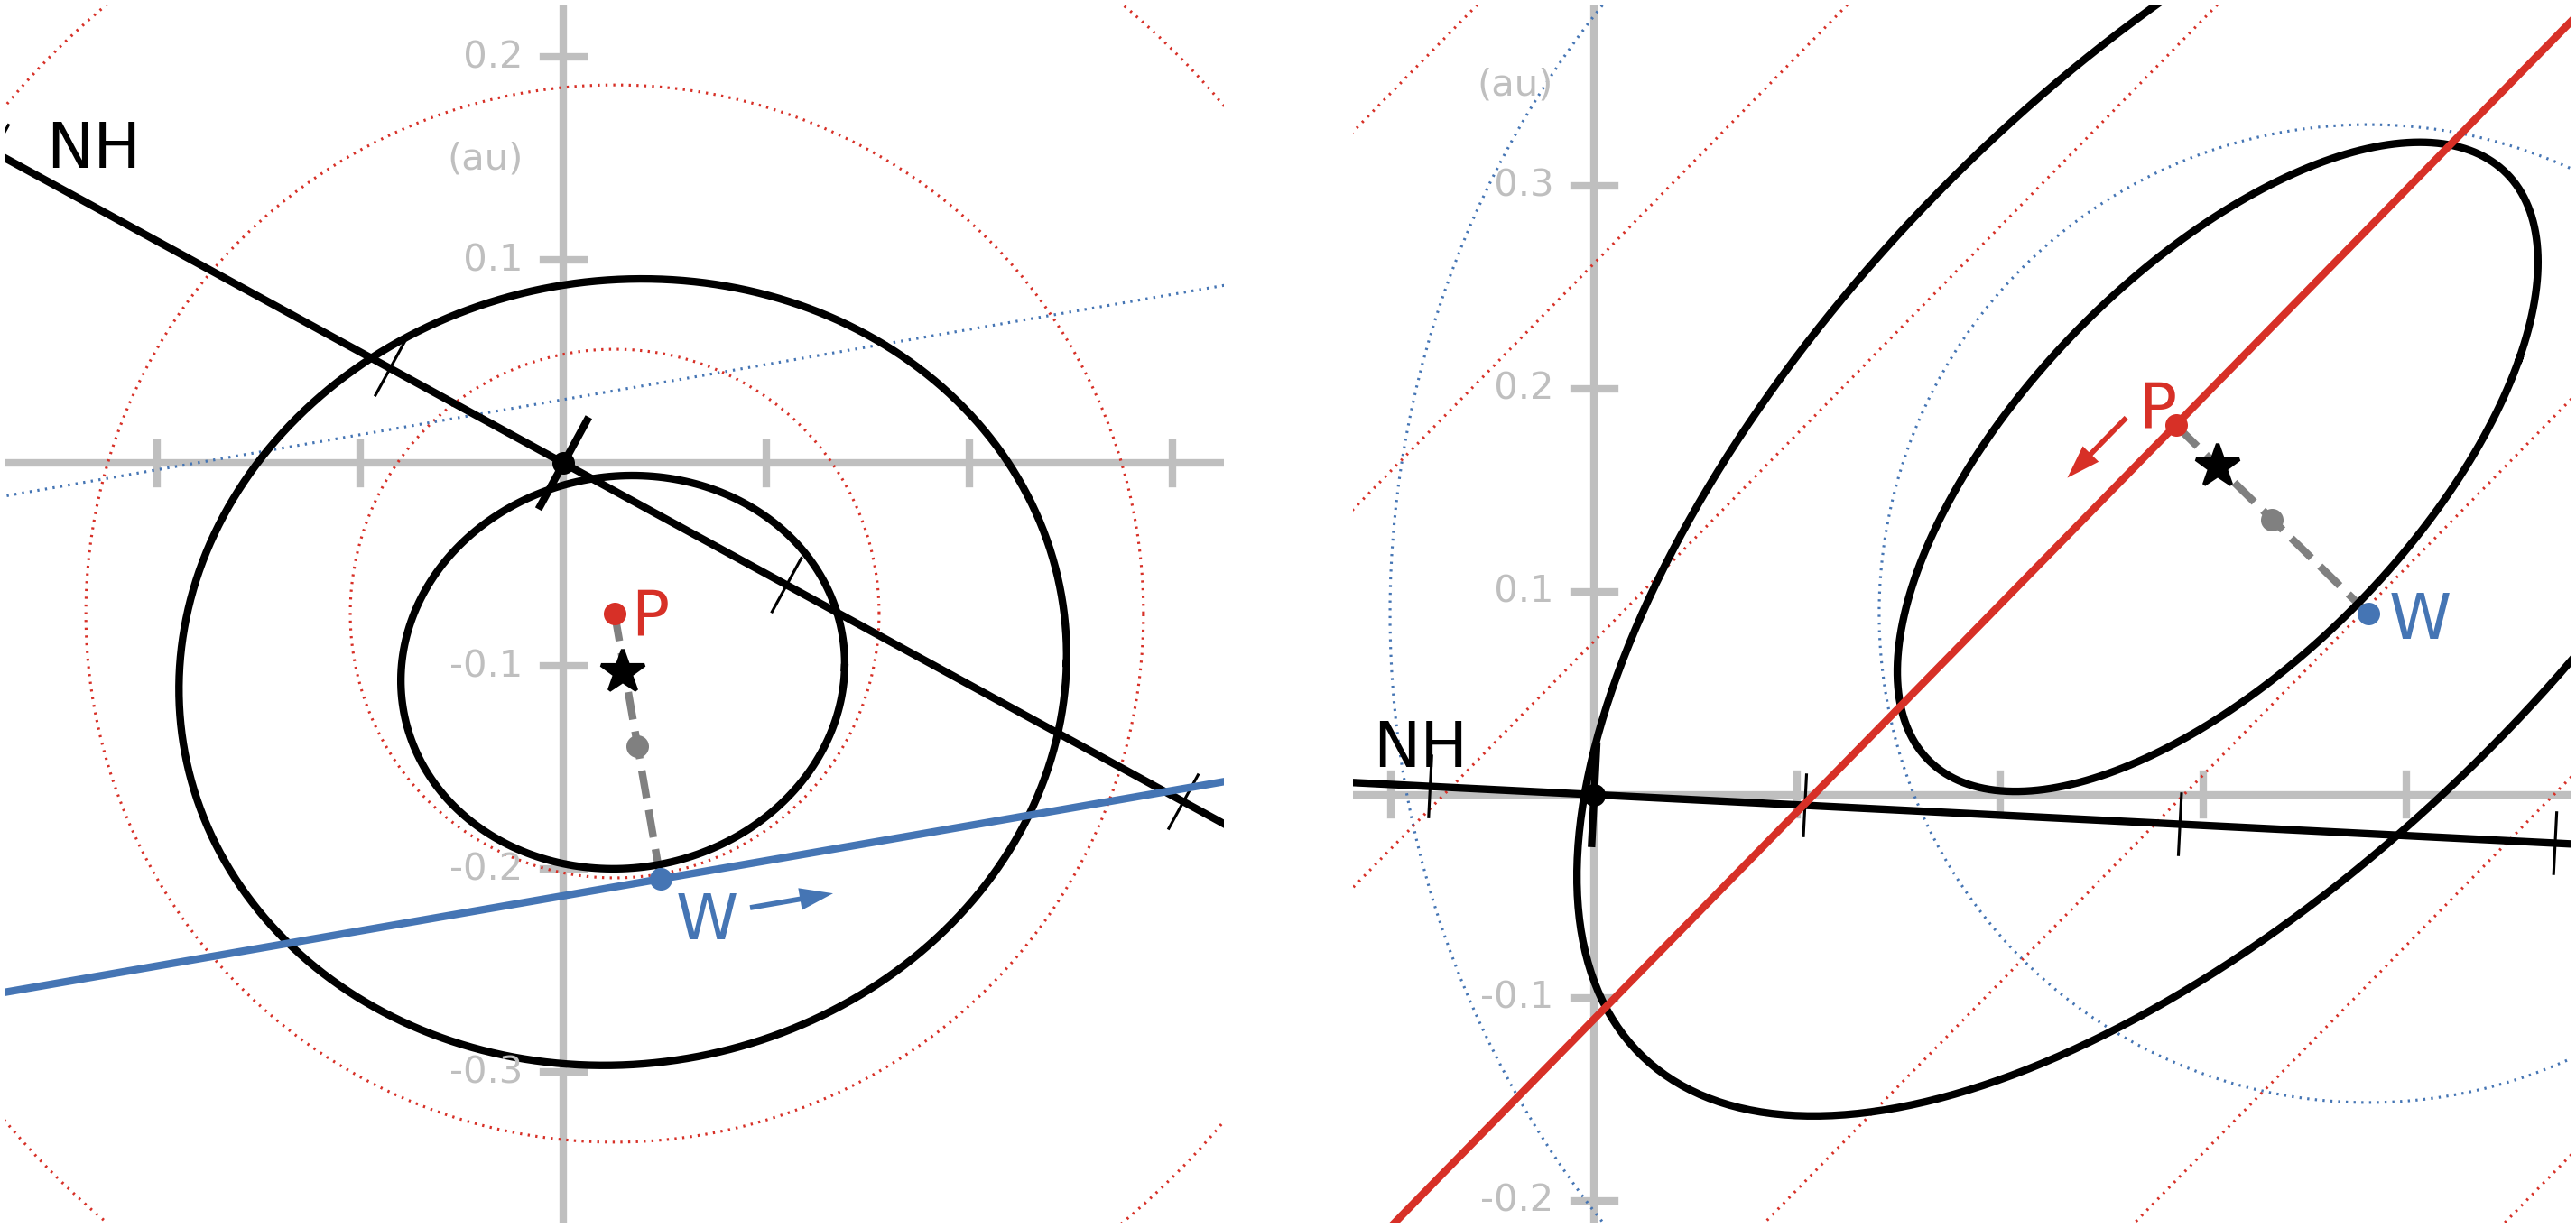
\includegraphics[keepaspectratio,width=7.0 in]{nhfig2.png}
\caption{Two zoomed views of the sight lines to Proxima Cen (P) and Wolf 359.  The left view is looking in the direction derived from LORRI images of Proxima Cen; the right view is looking in the direction derived from LORRI images of Wolf 359.  The NH line is the exact trajectory of New Horizons accordinag to JPL Horizons, with tick marks at 30 day intervals; the spacecraft is moving from right to left in both views.  The gray axes with ticks at 0.1 au intervals intersect at the position of NH on April 23, 2020.  The ticks on the trajectory before and after this point are April 5 and May 5, respectively.  The P and W lines are skew; the points of closest approach are connected by the dashed gray line, which lies in the plane of both drawings (ecliptic latitude is up in both views).  The lines are 0.133 au apart at closest approach.  The midpoint of the dashed connecting line is indicated by a gray dot.  The most likely spacecraft position $\BV{x}$ from Eq.(\ref{eq:x}) is indicated by the star.  It is 0.350 au from the true spacecraft position.  The faint dotted lines are nested cylinders around the P and W lines every $0''\!\!.1.$ The ellipses are the 1-sigma and 2-sigma error ellipses from Eq.(\ref{eq:xcov}) assuming $\sigma_\alpha=0''\!\!.2$ for each individual LORRI image.}
\label{fig:nav_zoom}
\end{figure}

For the case of two lines, it is clear that the minimum $\chi^2$ must occur on the shortest line segment connecting the two lines, which is the dashed gray line in Fig.(\ref{fig:nav_zoom}), because you could decrease the $\chi^2$ of any point off this line by zeroing its component perpendicular to the line.  This dashed line lies in the planes of both the left and right views; its direction is the cross product of the directions of the P and W lines.  The most likely point - the starred point - divides this connecting line into two parts with lengths in the ratio $p_1^2:p_2^2.$ Note that as the more distant star gets farther and farther away, the $\BV{x}$ from Eq.(\ref{eq:x}) rapidly converges on the line determined by the nearer star; at the same time, the error ellipse from Eq.(\ref{eq:xcov}) becomes more and more cigar shaped, aligned with the near star line.  This tendency is already evident in Fig.(\ref{fig:nav_zoom}) with Wolf 359 1.85 times farther away than Proxima Cen.

[Some version of Table 4 goes here, giving the positions of the JPL and solution points shown in Fig. 3.]

\end{document}
